\newcommand{\R}{ \mbox{${\Bbb R}$}}


\title{Probabilistic PCA}

\subsection{Probabilistic PCA}

Probabilistic PCA is useful when dealing with data that is dependent on both principal axes and latent variables \citep{tipping1999probabilistic}. It is often used when there are missing values in the data.

We'll run through a quick tutorial to implement it in Edward below. The full script can be accessed
\href{https://github.com/blei-lab/edward/blob/master/examples/probabilistic_pca.py}
{here}.

\subsubsection{Data}

We simulate our data points below. We'll talk about the individual variables and what they stand for in the next section. For this example, each point is 2-dimensional, $\mathbf{x}_n\in\mathbb{R}^2$.
\begin{lstlisting}[language=Python]
def build_toy_dataset(N, D, K, sigma=1):
  x_train = np.zeros((D, N))
  w = np.random.normal(0.0, 2.0, size=(D, K))
  z = np.random.normal(0.0, 1.0, size=(K, N))
  mean = np.dot(w, z)
  for d in range(D):
    for n in range(N):
      x_train[d, n] = np.random.normal(mean[d, n], sigma)

  return x_train

N = 5000  # number of data points
D = 2  # data dimensionality
K = 1  # latent dimensionality

x_train = build_toy_dataset(N, D, K)
\end{lstlisting}

This generates a dataset that looks like this:

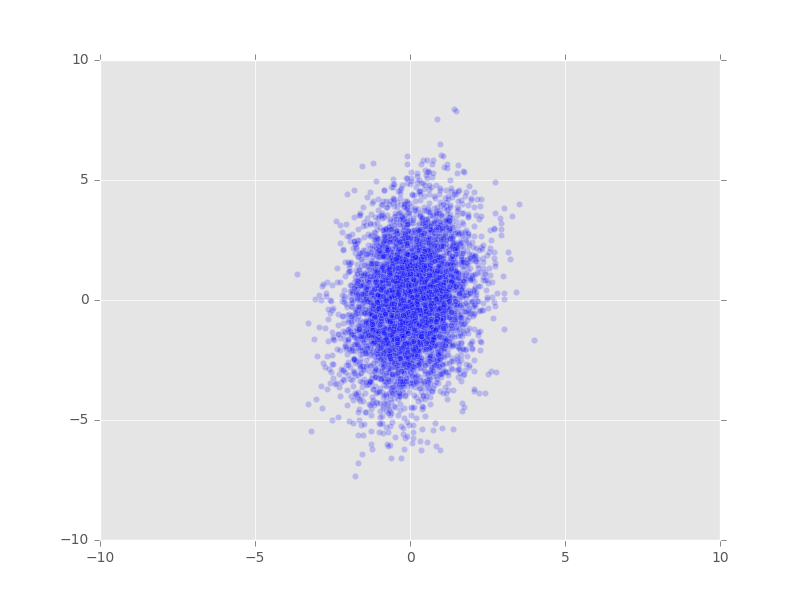
\includegraphics[width=450px]{/images/ppca-fig0.png}

\subsubsection{Model}

Consider a set of $N$ data points, $X = \{\mathbf{x}_n\}$ where $\mathbf{x}_n \in \Bbb{R}^D$.

While our data operates in dimension $D$, we will have latent variables $\mathbf{z}_n \in \Bbb{R}^K$ for every $\mathbf{x}_n$ such that $K < D$. The set of principal axes $\mathbf{W}$ relates our latent variables to our actual data.

Thus, we have that $$\mathbf{z} \sim N(0, \mathbf{I})$$ and that $$\mathbf{x} \vert \mathbf{z} \sim N(\mathbf{Wz} + \mu, \sigma^2\mathbf{I})$$ where $\mathbf{\epsilon} \sim N(0, \sigma^2\mathbf{I})$.

Because of the dependence on $\mathbf{Wz}$, we don't want to solely want to infer the original principal axes (as would be done in the vanilla PCA model). Rather, we aim to model the principal axes with respect to the latent variables.

For our marginal distribution, we get that $$x \sim N(0, \mathbf{W}\mathbf{W}^Y + \sigma^2\mathbf{I})$$

Note here that regular PCA is simply the specific case of Probabilistic PCA, as $\sigma^2 \to 0$.

We set up our model below by creating a prior distribution over our variables of interest so that we can infer the posterior.

\begin{lstlisting}[language=Python]
w = Normal(mu=tf.zeros([D, K]), sigma=2.0 * tf.ones([D, K]))
z = Normal(mu=tf.zeros([N, K]), sigma=tf.ones([N, K]))
x = Normal(mu=tf.matmul(w, z, transpose_b=True), sigma=tf.ones([D, N]))

\end{lstlisting}

\subsubsection{Inference}

Since $\mathbf{W}$ cannot be analytically determined, we must use some inference method. Below, we set up our inference variables and then run an approximation algorithm. For this example, our method is to minimize the $\text{KL}(q\|p)$ divergence measure.

\begin{lstlisting}[language=Python]
qw = Normal(mu=tf.Variable(tf.random_normal([D, K])),
            sigma=tf.nn.softplus(tf.Variable(tf.random_normal([D, K]))))
qz = Normal(mu=tf.Variable(tf.random_normal([N, K])),
            sigma=tf.nn.softplus(tf.Variable(tf.random_normal([N, K]))))

inference = ed.KLqp({w: qw, z: qz}, data={x: x_train})

init = tf.global_variables_initializer()
inference.run(n_iter=500, n_print=100, n_samples=10)
\end{lstlisting}

\subsubsection{Criticism}

One way to criticize the model is to visually compare our actual data to data produced by our inferred values. The blue dots represent the original data, while the red is the inferred.

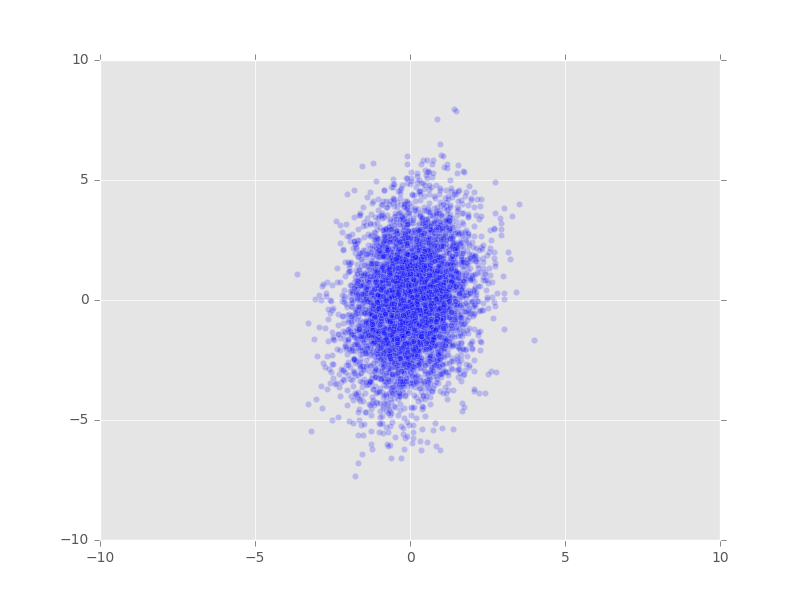
\includegraphics[width=450px]{/images/ppca-fig0.png}

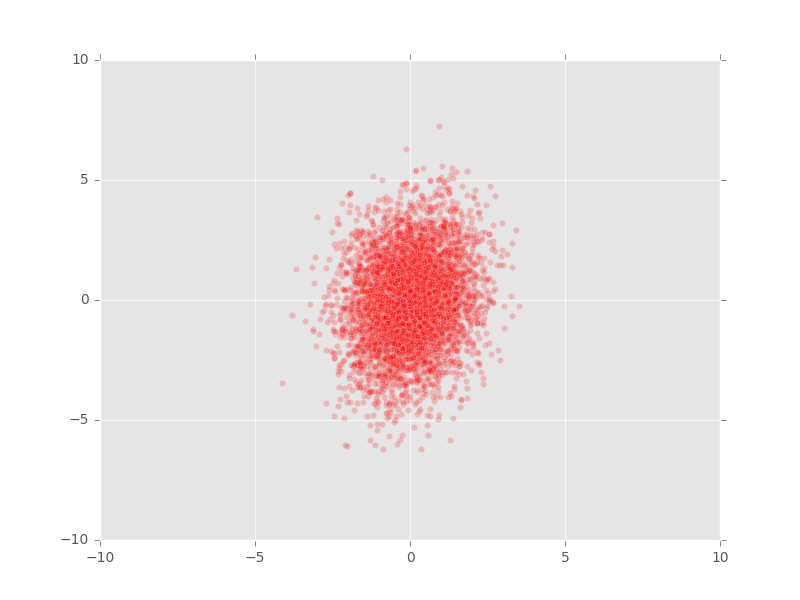
\includegraphics[width=450px]{/images/ppca-fig1.png}

\subsubsection{References}\label{references}
